\documentclass{acm_proc_article-sp}
\usepackage{graphicx}
\usepackage{algorithm}

\usepackage{algpseudocode}
\usepackage{amsmath}
\usepackage{graphics}
\usepackage{epsfig}

\begin{document}
\title{Source code analyzing with parallel programming technique}
\subtitle{NCTU Parallel programming 2015 Fall Final project}

\numberofauthors{3}
\author{
\alignauthor
Tseng Yi\\
       \affaddr{0356063}\\
       \affaddr{National Chiao Tung University}\\
\alignauthor
Wang Hsu Chien\\
       \affaddr{0356136}\\
       \affaddr{National Chiao Tung University}\\
\alignauthor
Chiang Sheng Yi\\
       \affaddr{0356549}\\
       \affaddr{National Chiao Tung University}\\
}

\date{1 19 2016}

\maketitle
\begin{abstract}
       This project shows that the performance improved while using multithread technique
       to analyzing million-line level source code like linux. Include line count, statement counting
       and function call recording.
\end{abstract}

\keywords{Parallel programming, pthread, code analyzing}

\section{Introduction}
\subsection{Background}
       Source code optimizing is one of key technique of compiler. 
       It's important to optimize source code for better performance, 
       less memory usage\ldots as so on. It's not enough by optimizing 
       source code by using compiler. We need to change the source 
       code and find the better way to implement our program. 
\subsection{Importance}
	By using simple analyzing program, we can find which statement we 
	use a lot, how many local variable we create, or how many useless 
	function we write. With those analyze data, developers can improve performance,
	decrease memory usage by reduce function calls or memory allocate.
\subsection{Motivation}
	However, it cost too much times to analyze source code while there
	exist a lots lines in our code, for example Linux kernel.
	We introduce a source code analyzer for million-line source code
	by using multi-thread technique, and compare the performance with 
	single thread analyzer.


\section{The problem}
\subsection{Performance of analyzing source code}
	There are a lot of ways to analyzing code, for example, calculate
	line number or statement number to let developer know the 
	volume of one program. We found that, there are many things that
	cause low performance for one program, such as increasing number 
	of recursive function call, or use less memory allocate.
	In this project, we want to calculate number of function calls and 
	number of \textbf{branch} statement like \textbf{if, switch, while, for}\ldots
	For single thread analyzer, if there are \textit{N} lines in one source file, 
	and there exist \textit{W} files in the project, assume that there only one 
	statement in one line, the time complexity is \textit{O(NW)}. Notice that
	NW is equals to total lines of the project.
	Next we need to figure out how to parse one line. The simplest way 
	to know which statement in specific line is using regular expression 
	and searching keywords, the time complexity of text searching is 
	\textit{O(TP)} where \textit{T} is length of text(line) and \textit{P} is length
	of pattern. Now we notice that each line, or file can be independent 
	if we only need to calculate specific statements or function calls, so
	we might improve performance by using parallel programming technique.

\section{Approach}
\subsection{Architecture of analyzer}
	Figure 1 shows the architecture of our program, there exist one dispatcher 
	and several analyzers, each analyzer will use one thread. Initially, the 
	dispatcher will scan all the project and create an index of all files, then
	it will generate multiple thread for analyzer. After generated thread, 
	dispatcher will send \textbf{block}s into analyzers.

\begin{figure}
	\centering
	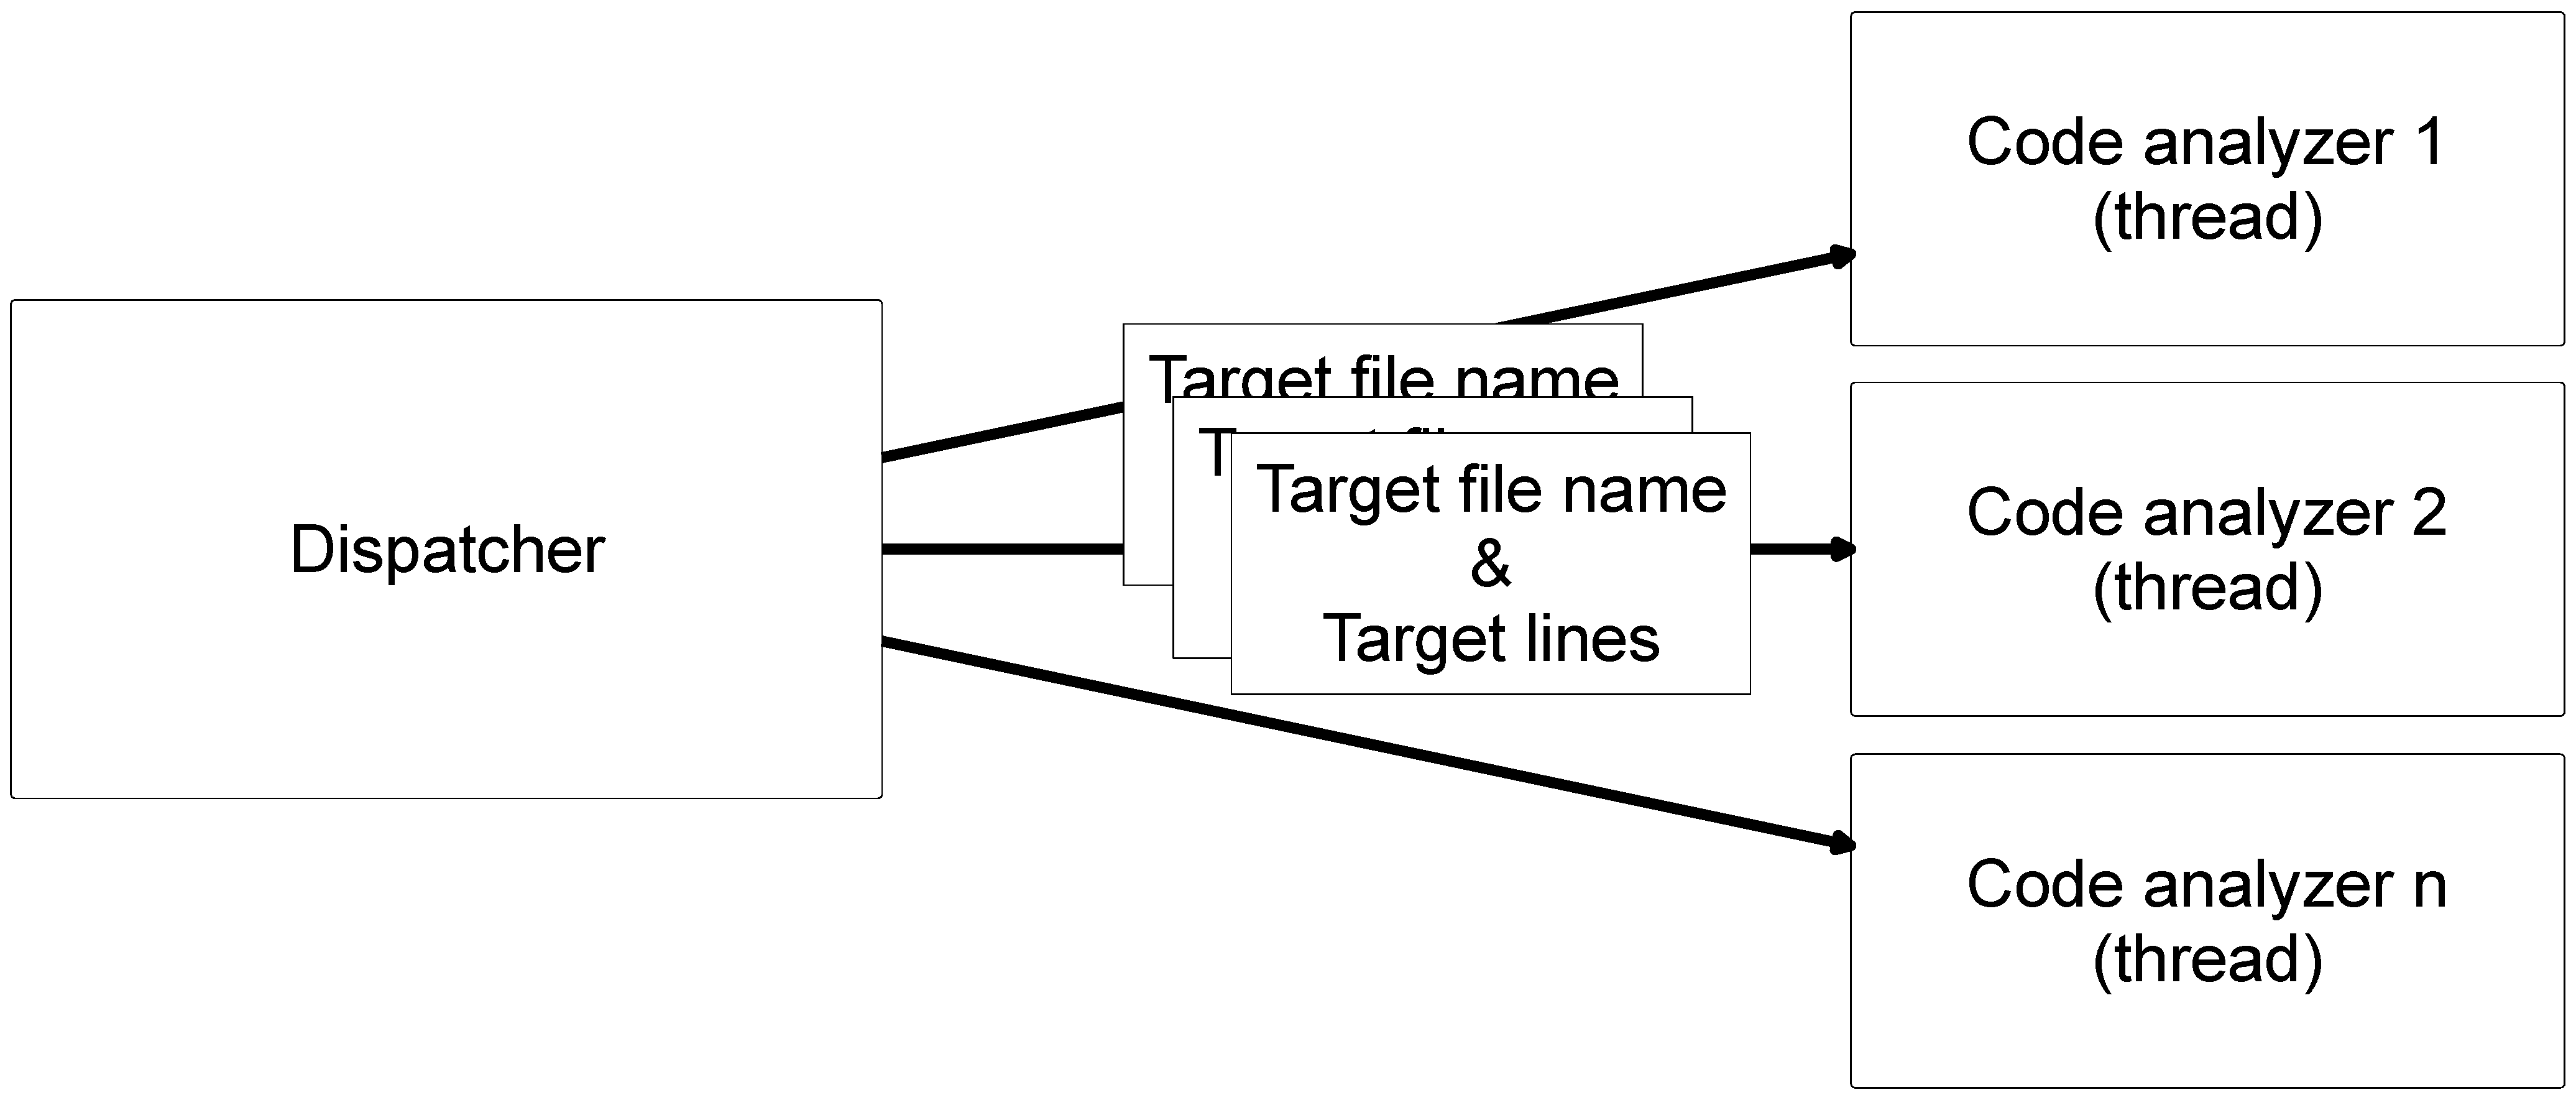
\epsfig{width=8cm, file=architecture.eps}
	\caption{Architecture}
\end{figure}


\subsection{Components}
\subsubsection{Dispatcher}
	The dispatcher will use list of source code files and convert all files into
	\textbf{block}s. Figure 2 shows that many source file split into many blocks
	, and dispatch into many analyzers. To find the ``cut'' point, first we need to 
	get total line of all source code, and divide it by number of thread(analyzer)
	that we need to use.
\begin{figure}
	\centering
	\epsfig{width=8cm, file=code_slice.eps}
	\caption{Slice source file into multiple blocks}
\end{figure}
\subsubsection{Code analyzer}
	Code analyzer will search specific pattern or syntax of one line, and record 
	it to it memory scope. There contains several functions in the analyzer:
	\begin{enumerate}
		\item Search \textbf{branch} statement like if, switch...
		\item Record function call
		\item Record number of statements(split by semicolumn)
	\end{enumerate}
	
\subsection{Workflow}
	Figure 3 shows the work flow of our program, there contains four part:
	\begin{enumerate}
		\item Scan: scan all file, recording number of lines of each file
		\item Dispatch: generate thread and send code blocks to it
		\item Analyze: analyze source code
		\item Merge: merge the result from analyzers
	\end{enumerate}

\begin{figure}
	\centering
	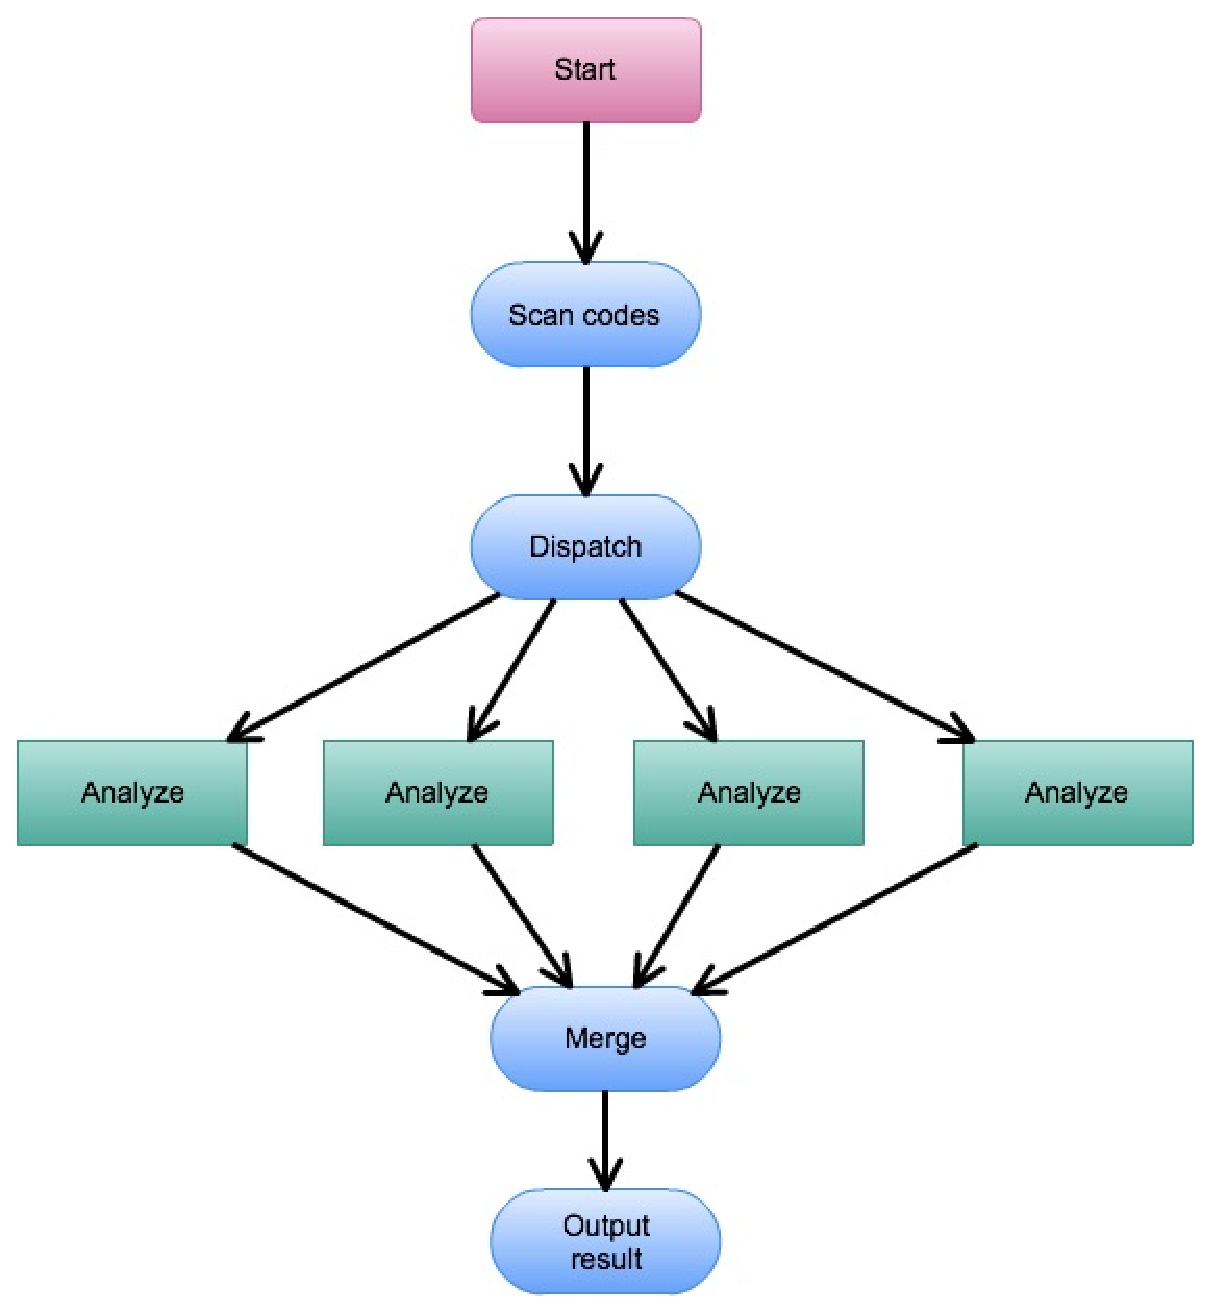
\epsfig{width=8cm, file=flow_chart.eps}
	\caption{Program workflow}
\end{figure}

\section{Language selection}
	In this project, we will use C++ with OpenMP multi-threading library.
	OpenMP (Open Multi-Processing) is an application programming interface 
	(API) that supports multi-platform shared memory multiprocessing 
	programming in C, C++, and Fortran. OpenMP is already built-in library in 
	C/C++ which is the language we are familiar with. OpenMP can be used on 
	various accelerators such as GPGPU. Original code statements do not 
	need to be modified when parallelized with OpenMP, this reduces the chance 
	of inadvertently introducing bugs. OpenMP does not need to deal with message 
	passing as MPI does. For the above reasons, OpenMP is a good choice for 
	out project.
	
\section{Proposed Solution}
\subsection{Single thread/process solution}
	To simply analyze code, we use \textit{regular expression}[4] to convert source
	code into \textbf{tokens}, and use these tokens to get information of each line
	of source code. For example, follow expression shows the regular expression of function call: 
	\begin{displaymath}
		[a-zA-Z_][a-zA-Z0-9_]+(.*);
	\end{displaymath}
	After convert code into tokens, we can record the number of each tokens. Also
	record function or variable names.
	Follow code is the basic algorithm of code analyzing.
	\begin{algorithm}[h]
		\caption{Single thread code analyze}
		\begin{algorithmic}[1]
			\Require
				$get\_token(x)$: parse code and get token list;
				$num\_lines$: total lines of source code;
				$s$: source code file pointer;
				$next\_line(s)$: get next line from source code;
			\State initial $current\_line=0$ and $token\_table is empty$;
			\While{$current\_line \ne num\_lines$}
				\State $line$ = $next\_line(s)$
				\State $token\_list$ = $get\_token(line)$
				\For{each $token \in $token\_list}
					\State $token\_table[$token]++
				\EndFor
				\State $current\_line$ = $current\_line + 1$
			\EndWhile
		\end{algorithmic}
	\end{algorithm}

\subsection{Multithread solution}
\subsubsection{Pthread}
	By using pthread, we create a single thread function to analyze one \textbf{block}
	of the source code. The argument of multi-thread function is the \textit{ID} of the thread.
	And we also pass \textbf{total lines of source code} and \textbf{number of threads} to
	thread function by using global variables.
	After the thread get it's ID, the thread calculate default \textit{width} of block, to calculate
	the width, simply use the equation below:
	\begin{displaymath}
	block\_width = \frac{number\_of\_lines}{number\_of\_threads}
	\end{displaymath}
	While the thread calculate the width of each block, calculate offset by using equation below:
	\begin{displaymath}
	block\_offset = thread\_id \times block\_width
	\end{displaymath}
	Each pthread thread function is like single thread program, the difference between single thread
	and multi-thread program is that multi-thread program contains a \textit{merge} state, we use
	global variable to store result data. To avoid race condition, we use different address of memory
	for different thread, thread will not access other thread's data. The following algorithm shows
	the progress for analyze source code by using pthread.
	\begin{algorithm}[h]
		\caption{Code analyze by using Pthread}
		\begin{algorithmic}[1]
			\Require
				$get\_token(x)$: parse code and get token list;
				$num\_lines$: total lines of source code;
				$thread\_id$: Thread ID;
				$num\_threads$: total number of threads;
				$s$: source code file pointer;
				$next\_line(s)$: get next line from source code;

			\Function {ANALYZE\_FUNC}{thread\_id}
				\State Initial $current\_line=0$ and $token\_table = empty$;
				\State $width = num\_lines \div num\_threads;$
				\State $offset = width \times thread\_id;$
				\State $current\_line = offset;$
				\While{$current\_line \ne offset + width$}
					\State $line$ = $next\_line(s)$
					\State $token\_list$ = $get\_token(line)$
					\For{each $token \in $token\_list}
						\State $token\_table[token] = token\_table[token] + 1;$
					\EndFor
					\State $current\_line = current\_line + 1;$
				\EndWhile
				\State $global\_token\_table[thread\_id] = token\_table;$
			\EndFunction
			\State Initial $global\_token\_table = empty table;$
			\For{$thread\_id \in \{0...num\_threads\}$}
				\State $craete\_thread(anal\_thread, thread\_id);$
			\EndFor
			\For{$thread\_id \in \{0...num\_threads\}$}
				\State $join\_thread(ANALYZE\_FUNC, thread\_id);$
			\EndFor
			\State Merge global\_token\_table;
		\end{algorithmic}
	\end{algorithm}

	
\subsubsection{OpenMP}
We have tried to parallel serial code of this project by using OpenMP. When we did homework 2, there were many for loop so we can easily use \textbf{\#pragma omp parallel for} to speed up many times. In this project, we have no for loop in serial code, so we divide the code that we want to analyze into n part (n, number of threads) and dispatch each part to the thread. We just use \textbf{\#pragma omp parallel} to let each thread do their task in parallel. The heaviest load in our project is the function named \textbf{get\_token()}. In order to avoid the race condition, we use one more dimension to store data from threads.
Follow code is the basic algorithm of code analyzing by using OpenMP.
\begin{algorithm}[h]
		\caption{Code analyze by using OpenMP}
		\begin{algorithmic}[1]
			\Require
				$get\_token(x)$: parse code and get token list;
				$num\_lines$: total lines of source code;
				$s$: source code file pointer;
				$num\_threads$: total number of threads;
				$next\_line(s)$: get next line from source code;
			\State initial $current\_line=0$ and $token\_table is empty$;
			\State Initiate OpenMP parallel loop
			\Repeat
				\State $line$ = $next\_line(s)$
				\State $token\_list$ = $get\_token(line)$
				\For{each $token \in $token\_list}
					\State $token\_table[$thread\_id][$token]++$
				\EndFor
				\State $current\_line$ = $current\_line + 1$
			\Until{$current\_line = num\_lines$}

			\For{each $token \in $token\_list}
			\Comment Synchronize data between slave thread to main thread
				\State $thread\_id = 0$
				\While{$thread\_id \ne num\_threads$}
					\State $token\_table_{token}$ = $token\_table_{token}$ + $parallel\_token\_table_{thread\_id\|token}$
				\EndWhile
			\EndFor
		\end{algorithmic}
\end{algorithm}

\subsubsection{MPI}
MPI is a language-independent communications protocol used for parallel programming. It's a message-passing application, and it's goals are high performance, scalability, and portability. 
First, should include the header files "mpi.h". At the begin of the program, need to Initialize MPI environment by this function "MPI\_Init". At the end of the program, need to terminate MPI execution environment by this function "MPI\_Finalize()".
Also, we use MPI\_Comm\_size to determine the size of the group associated with a communicator and MPI\_Comm\_rank to return the rank of calling process. After different parallel process deal with its work. MPI\_Reduce will combine the operands stored in the memory. It is a collective communication call where all the processes in a communicator.
\begin{algorithm}[h]
\caption{Code analyze by using MPI}
\begin{algorithmic}[1]
\Require
$get\_token(x)$: parse code and get token list;
$num\_lines$: total lines of source code;
$s$: source code file pointer;
$num\_threads$: total number of threads;
$next\_line(s)$: get next line from source code;
			\State initial $current\_line=0$ and $token\_table is empty$;
			\State initiate MPI
            \State $line$ = $next\_line(s)$
			\State $token\_list$ = $get\_token(line)$
			\If{parent process}
				\For {each $token \in $token\_list}
					\State $token\_table[$token]++
				\EndFor
			\EndIf
			\If{child processes}
				\For {each $token \in $token\_list}
					\State $token\_table[$token]++
				\EndFor
			\EndIf
			\State Reduce result by using MPI
		\end{algorithmic}
\end{algorithm}


\section{Experimental Methodology}
\subsection{Test}
	To test it, we encapsulated analyzer into one function, and use this function for different
	version of parallel method.
	Second, we deployed our source code into one single machine to ensure that the result
	is not affect by the environment.
	To calculate analysis time, we use \textbf{clock} system call to get current clock number
	and get another clock number after process finished. We use \textit{$clock_{end}$} - \textit{$clock_{start}$}
	to get execution time, and unit of time is clock.
\subsection{Input sets}
	We use Linux kernel[5] source code as our input. For reduce the complexity of testing
	and the dispatcher, we merge all of the code(.c and .h files) into one file. and we remove
	unused comment to ensure that there's no meaningless line.
	We randomly choose 850, 8500, 85000 and 850000 lines in the source code and pass
	it into our program by using standard input.
\subsection{Environment}
	The list below is out environment:
	\begin{enumerate}
		\item CPU: Intel(R) Xeon(R) CPU E3-1231 v3 @ 3.40GHz
		\item Cores: 8
		\item RAM: 16GB
		\item HDD: 256GB SSD
		\item OS: FreeBSD 10.1
	\end{enumerate}
	Also, we create new user for experiment to ensure that the environment is clean.

\section{Experimental Results}
\subsection{The results}
 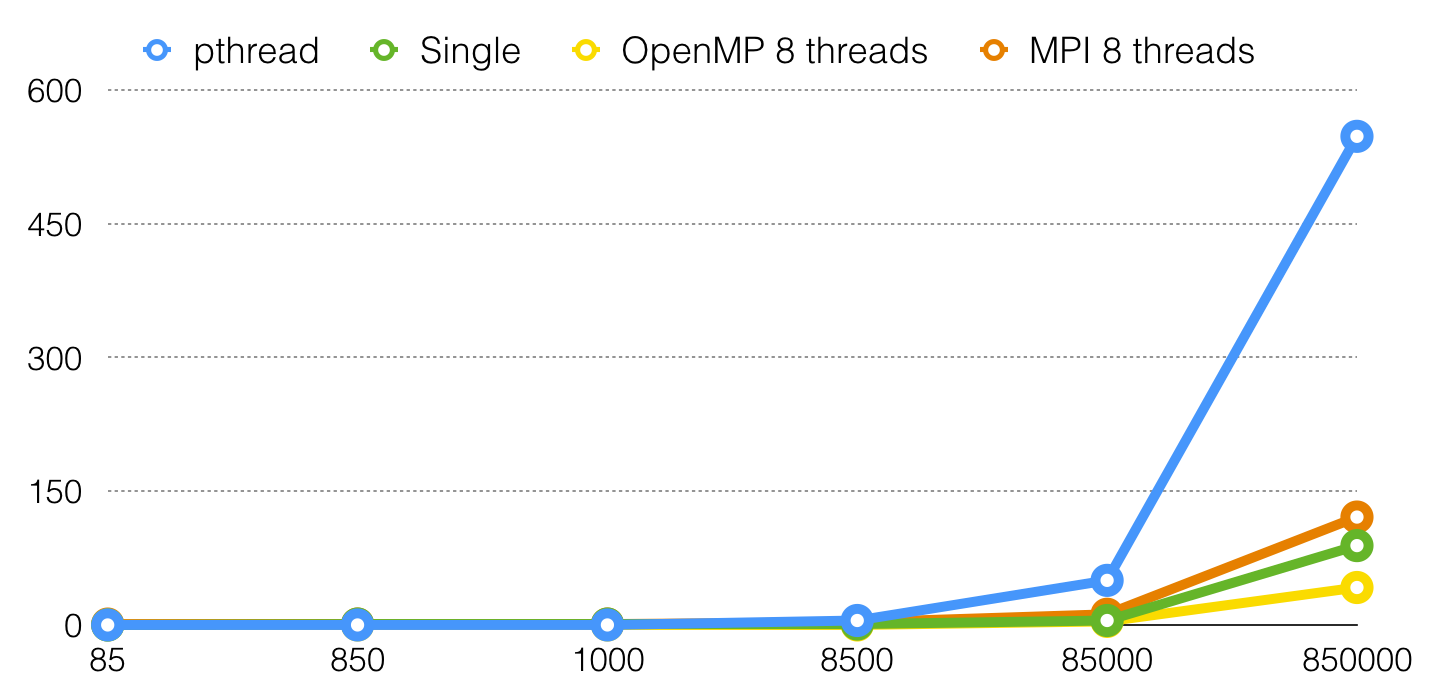
\includegraphics[width=8cm]{result.png}
\subsection{Analysis the low performance problem}

	
\section{Related work}

	\textbf{quantifiedcode}[3] provide online python code analyzer, it can let developer 
	know how to improve his/her code by giving some suggestions.
	nowadays, in multiple research, we can find that code analysis can be used to 
	detect malware software, this kind of static analysis take less resources and time. 
	It’s much easier than dynamic analysis method.

\section{Conclusions}


\section{References}
[1] OpenMP: 2015. http://openmp.org/wp/. Accessed: 2015- 11- 03.

[2] OpenMP wiki page : 2015. https://zh.wikipedia.org/zh-tw/OpenMP. Accessed: 2015- 11- 03.

[3] quantifiedcode : 2015. https://www.quantifiedcode.com/. Accessed: 2015- 11- 03.

[4] Regular expression

[5] Linux kernel

\end{document}
